
\appendix


\renewcommand{\thechapter}{A}
 \refstepcounter{chapter}
    \makeatletter
   \renewcommand{\theequation}{\thechapter.\@arabic\c@equation}
    \makeatother
\chapter*{\LARGE Appendix A\\\tiny\vspace{2\baselineskip}\LARGE Brief model formalism of the $pd\rightarrow ppn$ process}
\label{app_formalism}
\addcontentsline{toc}{chapter}{Appendix A: Brief model formalism of the $pd\rightarrow ppn$ process}






In the generalized eikonal approximation (GEA), the total amplitude of the process $pd\rightarrow ppn$ can be written in the following way (see Ref.~\cite{PhysRevC.107.014605} for details): \vspace{-0.3em} 
\begin{equation}
M_{\textrm{total}} = M_{\textrm{IA}} + \sum_{i}M_{\textrm{rescattering}}^{i},\label{eq:amplitude_tot}\\[-8pt]
\end{equation}
where $M_{\textrm{IA}}$ corresponds to the impulse approximation, i.e. to the situation when no rescattering of the initial/final protons off the spectator neutron takes place (no ISI/FSI), and $\sum_{i}M_{\textrm{rescattering}}^{i}$ is a combination of rescattering amplitudes that correspond to the case when initial/final protons rescatter off the spectator neutron. In Fig.~1 of Ref.~\cite{PhysRevC.107.014605}, $M_{\textrm{IA}}$ corresponds to the diagram (a), while $M_{\textrm{rescattering}}^{i}$ to all other diagrams, with the index $i$ running from (b) to (h).

For the two terms in Eq.~\eqref{eq:amplitude_tot}, the following is true\vspace{-0.3em} 
\begin{equation}
\begin{aligned}
M_{\textrm{IA}}&\sim M_{\textrm{hard}}^{\textrm{el}}\\
M_{\textrm{rescattering}}^{i}&\sim M_{\textrm{hard}}^{\textrm{el}}\cdot F_{i}\left(M_{\textrm{soft}}^{\textrm{el}}\right),\\[-8pt]
\end{aligned}\label{eq:amp_hard_soft}
\end{equation}

Here $M_{\textrm{hard}}^{\textrm{el}}$ is the hard elastic $pp$ scattering amplitude, which can be factorized out of the momentum integral, and $M_{\textrm{soft}}^{\textrm{el}}$ is the soft elastic $pn$ scattering amplitude, which is a part of the integrand of the momentum integral (and the function $F_{i}$ is specific to a particular rescattering amplitude).



Exact derivations for the $M_{\textrm{IA}}$ and $M_{\textrm{rescattering}}^{i}$ amplitudes can be found in Ref.~\cite{PhysRevC.107.014605}. Further calculations of the amplitudes rely on empirical parameterizations of $M_{\textrm{hard}}^{\textrm{el}}$ and $M_{\textrm{soft}}^{\textrm{el}}$, which are also available in Ref.~\cite{PhysRevC.107.014605}.


Based on the parameterization of the hard elastic $pp$ scattering amplitude $M_{\textrm{hard}}^{\textrm{el}}$, one can write this amplitude in the following form (see more details in Ref.~\cite{PhysRevC.107.014605}),\vspace{-0.3em} 
 \begin{equation}
M_{\textrm{hard}}^{\textrm{el}} = M_{\textrm{QC}} + M_{\textrm{L}},\label{eq:qc_Landshoff}
\end{equation}
where $M_{\textrm{QC}}$ stands for the ``Quark Counting" component that corresponds to the connected perturbative QCD graphs and is responsible for the formation of point-like configurations (PLCs), and $M_{\textrm{L}}$ stands for the Landshoff component that corresponds to the disconnected graphs and leads to conventional ISI and FSI of full-sized hadrons~\cite{Ralston:1988rb}.




The soft elastic $pn$ scattering amplitude $M_{\textrm{soft}}^{\textrm{el}}$ is parameterized in the standard high-energy form used in the Glauber theory. The full parameterization is available in Ref.~\cite{PhysRevC.107.014605}, and here, for simplicity, we write $M_{\textrm{soft}}^{\textrm{el}}$ in the following form,
\begin{equation}
M_{\textrm{soft}}^{\textrm{el}} = \xi \cdot \sigma_{pn}^{\textrm{tot}},\\[-8pt]\label{eq:soft_par}
\end{equation}
where $\sigma_{pn}^{\textrm{tot}}$ is the total cross section of the soft interaction between the final proton (that undergoes rescattering) and the spectator neutron ($p_{s}$ from Fig.~\ref{fig:diagram}), while the term $\xi$ contains all other factors of the parameterization.



To account for CT effects, the Quantum Diffusion Model (QDM) re-writes the $M_{\textrm{soft}}^{\textrm{el}}$ amplitude in a position dependent form~\cite{Farrar:1988me}, assuming that it depends on the variable $l$, which is the distance between a proton and a neutron in a deuteron along the momentum of a fast proton. The distance $l$ is defined in the deuteron rest frame as follows,\vspace{-0.3em} 
\begin{equation}
l = \frac{\left|\left(\overrightarrow{r_{2}} - \overrightarrow{r_{s}} \right)\cdot\overrightarrow{p}  \right|}{\left|\overrightarrow{p} \right|},\label{eq:l_distance}
\end{equation}
where $\overrightarrow{r_{2}}$ and $\overrightarrow{r_{s}}$ are the coordinate vectors of the intermediate proton and the spectator neutron ($p_{2}$ and $p_{s}$ from the left graph in Fig.~\ref{fig:diagram}), respectively, and $\overrightarrow{p}$ is the three-momentum of the nucleon that undergoes rescattering.

Note that based on Eqs.~\eqref{eq:amp_hard_soft} and~\eqref{eq:qc_Landshoff}, each of the rescattering amplitudes $M_{\textrm{rescattering}}^{i}$ is split into two terms: the first one is proportional to $M_{\textrm{QC}}$ and the second one is proportional to $M_{\textrm{L}}$. In the QDM, the CT contribution is included into the $M_{\textrm{soft}}^{\textrm{el}}$ amplitude of the term proportional to $M_{\textrm{QC}}$ and the $M_{\textrm{soft}}^{\textrm{el}}$ amplitude in the second term remains unchanged~\cite{Farrar:1988me,Ralston:1988rb}. 

The position dependence is introduced into the parameterization of the $M_{\textrm{soft}}^{\textrm{el}}$ amplitude (see Eq.~\eqref{eq:soft_par}) in the following form,\vspace{-0.6em} 
\begin{equation}
\left [ M_{\textrm{soft}}^{\textrm{el}}\right ]_{\textrm{QDM}} =\xi \cdot \sigma_{pn}^{\textrm{eff}} \cdot \frac{G\left (t \cdot \frac{\sigma_{pn}^{\textrm{eff}}}{\sigma_{pn}^{\textrm{tot}}}  \right)}{G(t)},\label{eq:soft_par2}
\end{equation}
where $G(t)$ is the Sachs electric form factor of a proton, $t$ corresponds to the momentum transferred in the soft $pn$ interaction, and $\sigma_{pn}^{\textrm{eff}}$ is defined by \vspace{-0.3em} 
\begin{equation}
\sigma_{pn}^{\textrm{eff}} =\mathcal F_{\textrm{CT}}(l)\cdot \sigma_{pn}^{\textrm{tot}},\label{eq:soft_par3}
\end{equation}
where $\mathcal F_{\textrm{CT}}(l)$ is a position dependent factor.


The QDM assumes that quark configurations appear at the hard interaction point with decreased size, which then gradually increases as the configuration travels away from this point. At distances $l\sim l_{\textrm{c}}$, the configuration expands to its ``normal" size, meaning that for $l\gtrsim l_{\textrm{c}}$, it interacts with the nuclear medium with the ``usual" cross section. Here $l_{\textrm{c}}$ is the so-called coherent length, which is defined as
\begin{equation}
l_{\textrm{c}} = \frac{2\left|\overrightarrow{p} \right|}{\Delta M^{2}},\label{eq:l_coh}
\end{equation}
where $\Delta M^{2}$ is the free parameter of the QDM and $\left|\overrightarrow{p} \right|$ was defined in the context of Eq.~\eqref{eq:l_distance}.



This situation is illustrated in Fig.~\ref{fig:l_coh}, where the factor $\mathcal F_{\textrm{CT}}$ is plotted as a function of the variable $l$. As $l$ grows from zero, the factor increases from its minimal value until it reached unity at $l = l_{\textrm{c}}$, and then stays at this value for $l> l_{\textrm{c}}$. The part of the graph shown by the dashed line (for $l<l_{\textrm{c}}$) corresponds to the color transparency regime, where a quark configuration interacts with the nuclear medium with the reduced cross section.  

\begin{figure}[htp]
\begin{center}
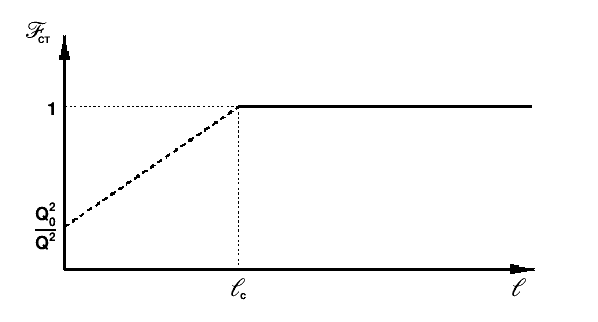
\includegraphics[width=0.67\textwidth]{pictures/l_coh.png}
\caption{\small The position dependent factor $\mathcal F_{\textrm{CT}}$, through which CT effects are introduced into the parameterization of the $M_{\textrm{soft}}^{\textrm{el}}$ amplitude in the QDM (see Eqs.~\eqref{eq:soft_par},~\eqref{eq:soft_par2},~and~\eqref{eq:soft_par3}). The factor is plotted as a function of the variable $l$ defined by Eq.~\eqref{eq:l_distance}. The coherence length $l_{\textrm{c}}$ is calculated according to Eq.~\eqref{eq:l_coh}. The part of the graph shown by the dashed line (for $l<l_{\textrm{c}}$) corresponds to the color transparency regime, where a quark configuration interacts with the nuclear medium with the reduced cross section. See text for more details.   } \label{fig:l_coh}
\end{center}
\end{figure}


Note that smaller values of the factor $\mathcal F_{\textrm{CT}}$ indicate larger CT effects and $\mathcal F_{\textrm{CT}} = 1$ corresponds to the absence of CT effects. This means that CT effects are more pronounced for larger values of the momentum transferred $Q^{2}$ and also for the case when larger values of the coherence length $l_{\textrm{c}}$ are available.



As follows from Eq.~\ref{eq:l_coh}, the coherence length $l_{\textrm{c}}$ is proportional to the momentum of the final proton (the one that undergoes rescattering). For higher collision energies ($\sqrt{s}$), larger values of the final proton momentum are accessible, meaning that CT effects are more pronounced for higher $\sqrt{s}$.

The minimal value of the factor $\mathcal F_{\textrm{CT}}$ is observed at $l=0$ and is equal to $\frac{Q^{2}_{0}}{Q^{2}}$ (here $Q^{2}_{0}=\langle n^{2}k_{t}^{2}\rangle$ with $n=3$ being the number of valence quarks in the proton and $\sqrt{\langle k_{t}^{2}\rangle}= 0.35$~GeV/c the average transverse momentum of a quark in a proton). This minimal value reflects how small the quark configuration was upon its formation at the hard interaction point and depends on the value of the momentum transferred $Q^{2}$. This means that CT effects are more pronounced for larger $Q^{2}$.


\newpage

In the QDM, CT effects are introduced through the position-dependent factor $\mathcal F_{\textrm{CT}}$.

The QDM assumes that quark configurations appear at the hard interaction point with decreased size, which then gradually increases as the configuration travels away from this point. At distances $l\sim l_{\textrm{c}}$, the configuration expands to its ``normal" size, meaning that for $l\gtrsim l_{\textrm{c}}$, it interacts with the nuclear medium with the ``usual" cross section. Here $l$ is the distance between a proton and a neutron in a deuteron along the momentum of a fast proton and $l_{\textrm{c}}$ is the so-called coherent length.


The simulation was performed in the following kinematic area, $\sqrt{s}=13$~GeV, $\alpha_{s} =1$ with $\Delta \alpha_{s} = 0.25$, $t=-6.8$~GeV$^2$ (which corresponds to $\theta_{\textrm{c.m.}}=49^{o}$) with $\Delta t = 2.5$~GeV$^{2}$, $\Delta \phi = 2\pi$, and $0.1$~GeV/c~$<p_{st}<0.5$~GeV/c.

